%%%%%%%%%%%%%
\chapter{Ergebnisdiskussion}
\label{ch:Results}
%%%%%%%%%%%%%
Zur Bewertung der Konzepte werden die in Kapitel \ref{ch:evaluation} beschriebenen Daten zunächst interpretiert. Die Ergebnisse der Interpretation werden anschließend kritisch betrachtet und, basierend auf der Ergebnisinterpretation, ein Ausblick der nächsten Schritte, für die Umsetzung des \emph{TMA} beschrieben. 


\section{Ergebnisinterpretation}
Die Ergebnisinterpretation erfolgt auf den, in Kapitel \ref{ch:evaluation}, aufgestellten Hypothesen. Ziel der Ergebnisinterpretation ist darzulegen, dass ein Modellierungsansatz nach dem Konfigurationsprinzip für den späteren Anwender verständlicher ist. Als Baseline dient hierfür das \emph{movisensXS}-System, welches ein Konstruktionsprinzip verfolgt. Dieser Ansatz bietet im Vergleich sehr viel Flexibilität in der Gestaltung einer Therapie. Die Ergebnisse werden kategorisiert betrachtet. Gegenübergestellt werden jeweils, wie bisher, das Konstruktionsprinzip und Konfigurationsprinzip, sowie der Einsatz von Sprüngen und die Verwendung von Sichtbarkeitsregeln. Die Betrachtung der Ergebnisse wird gemäß der zuvor verwendeten Reihenfolge erfolgen. Abschließend werden die Ergebnisse zusammengefasst dargestellt.

 
\begin{figure}[h]
\centering
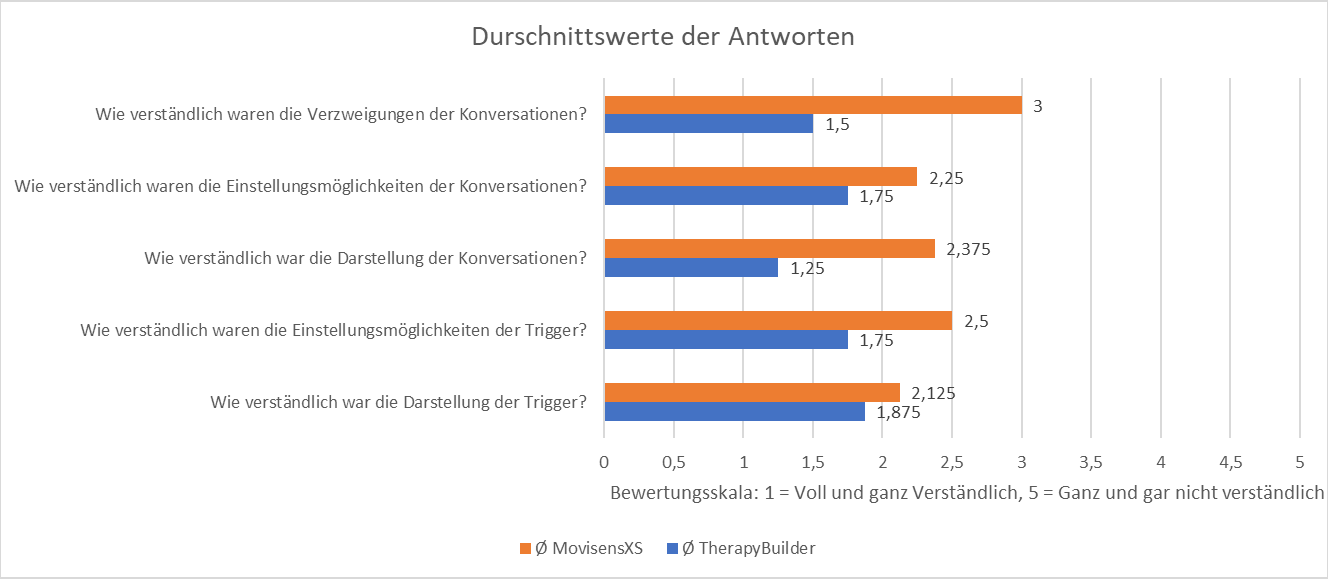
\includegraphics[width=1\textwidth]{pictures/diagramme/antwortendurchsch1}
\caption{Architektur des \emph{konfiguration}}
\label{antwortendurchsch11}
\end{figure}

\begin{figure}[h]
\centering
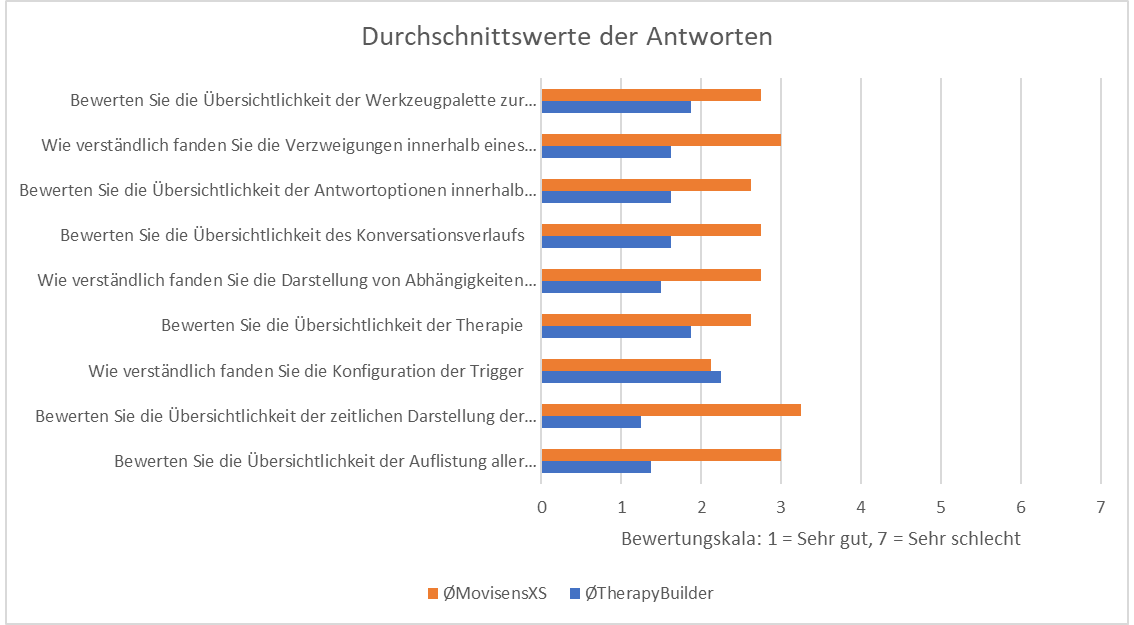
\includegraphics[width=1\textwidth]{pictures/diagramme/antwortendurchsch2}
\caption{Architektur des \emph{konfiguration}}
\label{antwortendurchsch22}
\end{figure}


\subsection{Konfigurationsprinzip und Konstruktionsprinzip}
Eine erste Betrachtung der Ergebnisse, deutet darauf hin, dass die Nutzer die Umsetzung und Verwendung des Konfigurationsprinzips besser bewerteten als das Konstruktionsprinzip. Wie in Abbildung \ref{antwortendurchsch11} und Abbildung \ref{antwortendurchsch22} zu sehen ist, haben die Probanden den \emph{TherapyBuilder}-Prototyp im Schnitt besser bewertet als das angepasste \emph{movisensXS}-System. Diese Ergebnisse wurden den Zwischenfragebögen entnommen und zeigen eine erste Tendenz auf. 

Auch die Ergebnisse der Abschlussfragerunde geben einen ersten Hinweis auf die Bewertung der Verständlichkeit und Übersicht beider Prinzipien. Insgesamt konnten die Probanden in der Abschlussfragerunde achtundzwanzig Punkte nennen (vgl. Abbildung \ref{konstrabsch} und \ref{konfigabsch}), die ihnen am Konstruktionsprinzip gut gefallen haben und die sie besonders hilfreich empfanden. Zum Konfigurationsprinzip äußerten sie hierzu hingegen neununddreißig Punkte. Die Probanden konnten somit bezüglich des Konfigurationsprinzips insgesamt mehr Punkte äußern, die ihnen an dieser Umsetzung gut gefallen haben und besonders hilfreich empfunden wurden. Betrachtet man diese jedoch im Einzelnen, wurden Konstruktionsprinzip mehr Punkte dahingehend geäußert, was den Probanden gut gefallen hat. Hinsichtlich der Nachfrage, was den Probanden an der jeweiligen Umsetzung nicht gefallen hat und was sie vermisst haben, schnitt auch hier das Konfigurationsprinzip besser ab. Im Vergleich zum Konstruktionsprinzip fielen den Probanden neunzehn Punkte ein. Das sind dreizehn Punkte weniger als die Probanden zum Konstruktionsprinzip äußerten. Zwar gibt es insgesamt mehr positive Anmerkungen bezüglich des Konfigurationsprinzip, allerdings wurden gegenüber dem Konstruktionsansatz mehr Punkte genannt, die den Probanden an diesem Ansatz besonders gut gefallen haben. Welche Punkte das sind und wie sich diese mit den Ergebnissen und aufgestellten Hypothesen verbinden lassen, wird im Verlauf dieses Kapitels betrachtet.


\begin{figure}
   \begin{minipage}[b]{.49\linewidth} % [b] => Ausrichtung an \caption
      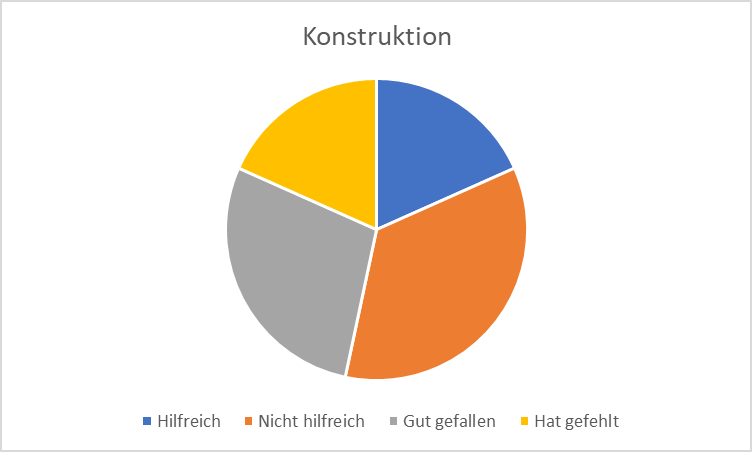
\includegraphics[width=\linewidth]{pictures/diagramme/aussagenkonstr}
      \caption{Zu sehen ist die Anzahl der genannten Punkte der Abschlussfragerunde. Die Probanden nannten achtundzwanzig Punkte auf die Frage was ihnen am Konstruktionsprinzip gut gefällt und sie als hilfreich empfinden}
      \label{konstrabsch}
   \end{minipage}
   \hspace{.01\linewidth}% Abstand zwischen Bilder
   \begin{minipage}[b]{.49\linewidth} % [b] => Ausrichtung an \caption
      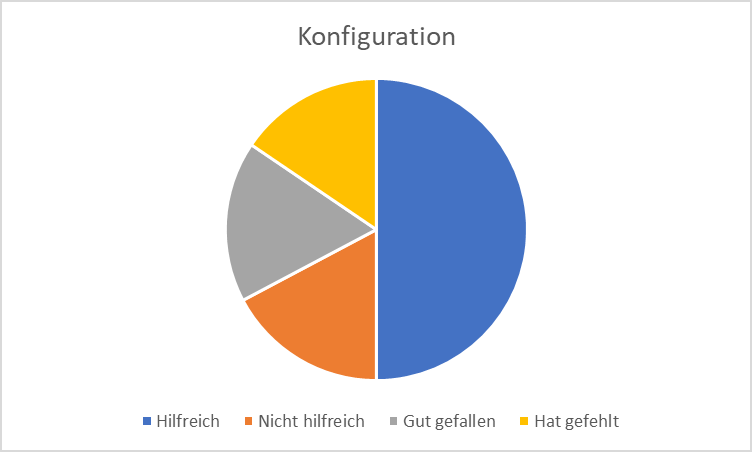
\includegraphics[width=\linewidth]{pictures/diagramme/aussagenkonfig}
      \caption{Im Vergleich äußerten die Probanden deutlich mehr Punkte, die sie am umgesetzten Konfigurationsprinzip als hilfreich empfinden. Allerdings konnten sie auch weniger Aussagen darüber treffen, was ihnen besonders gut gefallen hat}
      \label{konfigabsch}
   \end{minipage}
\end{figure}



\paragraph{Verständlichkeit der Triggereinstellungen}
Die Ergebnisse der Zwischenfragebögen zeigen eine Tendenz, dass im Vergleich das Kontruktionsprinzip für Anwender verständlicher ist. Die Freitexte der Zwischenfragebögen und Abschlussfragerunde deuten hingegen darauf hin, dass zwar viele Einstellungsmöglichkeiten geboten werden ohne mit diesen zu erschlagen und gefühlt weniger Einstellungsschritte und notwendig sind. Der Fluss vom Klicken wirkt klarer und konsistenter. Allerdings äußerten mehrere Probanden, dass die Einstellungen der Trigger zunächst irritierten. Betrachtet man die Ergebnisse der Abschlussfragerunde bestätigt sich letztere Aussage. Die Hälfte der Probanden wünschen sich eine Anleitung oder Tooltips zum besseren Verständnis der Triggereinstellungen.

Zwar wurde das \emph{movisensXS}-System im Zwischenfragebogen hinsichtlich der Triggereinstellungen schlechter bewertet. Dennoch kann das verwendete Konstruktionsprinzip mit seiner flexiblen Gestaltungsmöglichkeit aufwarten. Die Einstellungen der Trigger werden bei wachsender Komplexität unübersichtlicher. Aber insbesondere die vielen Einstellungsmöglichkeiten via Drag and Drop durch das Baukastenprinzip, und die Flexibilität in der Anordnung und Gestaltung, sind generell besser nachvollziehbar. Nicht nur das Baukastenprinzip und die einhergehende Drag and Drop Funktion tragen dazu bei, sondernm auch die Trennung verschiedener Elemente anhand ihrer Funktion. 

Insgesamt ist zwar eine Tendenz gegeben, dass das Konstruktionsprinzip leichter verständlich ist, allerdings benötigt dieses zusätzlich Anleitungen und Tooltips um diese zu verbessern. Auch wenn das Konstruktionsprinzip tendenziell schlechter abschneidet, so ist gerade das zusammenbauen der Triggereinstellungen für die Nutzer interessant und das Prinzip an sich leicht nachvollziehbar. Allerdings kann hier auch die flexible Anordnung zu einer geringeren Übersicht beitragen. Hier könnte eine automatische Anordnungsfunktion, oder Anordnungshilfe zur besseren Übersicht beitragen.


\paragraph{Verständlichkeit der Triggerdarstellung}
Auch hier lässt sich in Abbildung \ref{antwortendurchsch11} eine leichte Tendenz erkennen, dass die Triggerdarstellung im Konfigurationsprinzip verständlicher ist. Der Unterschied zwischen dem Konstruktionsprinzip und Konfigurationsprinzip ist hier allerdings relativ gering. Insbesondere die zeitliche Übersicht und das Zusammenbringen der Einstellungen und dem Ablauf empfanden die Probanden als positiv. Allerdings kristallisiert sich heraus, dass die Farben zwar zur Übersicht beitragen. Nur eine Erklärung dessen fehlt zum besseren Verständnis. Generell wurde die Darstellung zwar als übersichtlich beschrieben, aber die Verständlichkeit leidet unter den fehlenden Erläuterungen zu den angebotenen Farben, Symbolen und anderen Darstellungsformen. 

Das Konstruktionsprinzip hingegen wird zwar in der Darstellung schnell unübersichtlich, aber besonders die Farben der einzelnen Bausteine helfen beim Orientieren. Außerdem beinhaltet die Darstellung mehr Informationen auf einem Blick. Besonders die farbliche Kodierung der Blöcke wird von den Probanden positiv hervorgehoben. 

Zwar schneidet das Konfigurationsprinzip besser ab, allerdings nur geringfügig. das Konstruktionsprinzip hebt sich besonders durch die farbliche Kodierung hervor. Diese Eigenschaft kann sich das Konfigurationsprinzip zu eigen machen. Eine durchdachte farbliche Kodierung der Trigger in Kombination mit entsprechenden Symbolen und einer ausführlichen Legende mit Erklärungen, können erheblich zu einer verständlicheren Darstellung der Trigger beitragen. Auch das hinterlegen von Informationen über die Triggereinstellungen, in Form von Tooltips an den zeitlich dargestellten Elementen, können sich positiv auf das Konfigurationsprinzip auswirken. Auch hier kann das Konstruktionsprinzip von einer strikteren Anordnungsvorgabe profitieren. 

\paragraph{Übersichtlichkeit der Konversationen}
Betrachtet man die erhobenen Daten hinsichtlich der Übersichtlichkeit innerhalb der verschiedenen Konzepte, so lässt sich auch hier eine Tendenz erkennen. Wie in Abbildung \ref{antwortendurchsch22} zu sehen, schneidet das Konfigurationsprinzip des \emph{TherapyBuilders} besser in der Fragebogenauswertung ab als das Konstruktiosnprinzip. Die Tendenz zeigt, dass die Listendarstellung aller Konversationen innerhalb der Darstellung des Konfigurationsprinzip, übersichtlicher gestaltet ist, als die freie Anordnung innerhalb des Konstruktionsprinzips des \emph{movisensXS}. Die Ergebnisse der Abschlussfragerunde bekräftigen die Ergebnisse des Fragebogens. Besonders die Listendarstellung und die hierfür angebotene Suchmöglichkeit nach einzelnen Konversationen werden als positive Punkte angebracht. Diese wird im Konstruktionsprinzip hingegen vermisst. Will der Nutzer eine Konversation und dessen Triggereinstellungen betrachten, muss diese erst im Baum gesucht werden. 

Triggereinstellungen einer Konversation einzusehen, gestaltet sich im Konfigurationsprinzip tendenziell leichter. Eine Suchfunktion könnte das Konstruktionsprinzip in diesem Punkt verbessern.


\paragraph{Übersichtlichkeit der zeitlichen Darstellung der Konversationen}
Abbildung \ref{antwortendurchsch22} verdeutlicht die unterschiedliche Bewertung beider Systeme hinsichtlich ihrer zeitlichen Darstellung der Konversationen. Es zeichnet sich eine deutliche Tendenz ab, dass diese innerhalb des Konfigurationsprinzips eine bessere Übersicht über die zeitliche Steuerung der Konversationen besteht. Die Ergebnisse der Freitexte, sowie der Abschlussfragerunde, untermauern das Ergebnis. So ist der zeitliche Ablauf und die Darstellung im Zeitstrahl übersichtlich, leicht nachvollziehbar. Außerdem lässt sich die spätere Belastung des Patienten einsehen. Alle Probanden äußerten sich positiv über diese Art der Darstellung. Ein Proband vermisst allerdings Funktionen bei dieser Darstellung. So wünscht sich dieser eine Möglichkeit auf einzelne Elemente zu klicken und eine Funktion damit auszulösen. Hingegen wurde das Konstruktionsprinzip in diesem Punkt ausschließlich kritisiert. Der zeitliche Ablauf der Konversationen ist schwer zu überblicken. 

Das Konfigurationsprinzip kann leicht um den Punkt der klickbaren Elemente und einer dahinter versteckten Funktion, wie beispielsweise das Aufrufen der Trigger-Einstellungen, erweitert werden. Um das Konstruktionsprinzip in diesem Punkt zu verbessern, könnte eine stärkere Vorgabe für die Strukturierung und Anordnung der Elemente auf dem entsprechenden Arbeitsblatt hilfreich sein. So könnte auch eine zeitliche Abfolge der Konversationen dargestellt werden.


\paragraph{Verständlichkeit der Triggerkonfiguration}
Hinsichtlich der Konfigurierung der Trigger wurde der \emph{TherapyBuilder}-Prototyp schlechter bewertet als der \emph{movisensXS}-Prototyp. Es ist eine Tendenz erkennbar, die aufzeigt, dass das Konstruktionsprinzip hinsichtlich der Triggerkonfiguration verständlicher ist. Die Betrachtung der Freitext-Aussagen sowie der Abschlussfragerunde geben Hinweise, in welchen Punkten sich das Konstruktionsprinzip hervorhebt. So ist insbesondere die Anordnung der Bausteine leicht verständlich. Die Drag and Drop Funktion erleichtert diese außerdem. Die einhergehende Flexibilität der Anordnung, sowie die farbliche Kodierung der Bausteine fallen positiv auf und tragen der Verständlichkeit bei. Diese wird beim Konfigurationsprinzip vermisst. So sind die Einstellungen der Konditionen nicht ganz klar. Außerdem lässt sich die Bearbeitungsfunktion der Trigger schwer finden. 

Um die Konfiguration der Trigger des Konfigurationsprinzip verständlicher zu gestalten, benötigt es zunächst einen besseren Zugang zu den Einstellungen. Außerdem sollten die Funktionen und Einstellungen erneut überarbeitet werden. Hier könnte eine strengere Form des Konstruktionsprinzips verwendet werden um die Einstellungsmöglichkeiten flexibel und verständlich zu gestalten. Möglich wäre eine Vorgabe von kleinen Bausteinen, die beliebig angeordnet, farblich kodiert und eingestellt werden können, sich allerdings nur auf eine Konversation bezieht, statt, wie im Konstruktionsprinzip, auf beliebig viele. Diese Form könnte die Übersichtlichkeit des Konfigurationsprinzip beibehalten.


\paragraph{Verständlichkeit von Abhängigkeiten zwischen Konversationen und Konversationsverzweigungen}
Die Abhängigkeiten zwischen Konversationen ist im Vergleich zum 
Die Grafiken \ref{antwortendurchsch11} und \ref{antwortendurchsch22} verdeutlichen eine positive Tendenz hinsichtlich der Verständlichkeit von Konversationsverzweigungen und Abhängigkeiten zwischen Konversationen im \emph{TherapyBuilder}. Das dort eingesetzte Konfigurationsprinzip wird in diesem Punkt allerdings kaum in den Freitext-Aussagen sowie der Abschlussfragerunde erwähnt. Nur zwei Probanden äußern, dass die Darstellung der Abhängigkeiten gut einsehbar sind. Der \emph{movisensXS}-Prototyp wird generell als weniger übersichtlich und verständlich bezüglich des zeitlichen Verlaufs beschrieben. Allerdings geht auch hier kein Proband genauer auf die Abhängigkeiten zwischen Konversationen ein. 

Generell könnte das Konstruktionsprinzip des \emph{TherapyBuilder} auch in diesem Punkt durch eine verständliche und ausführliche Legende, sowie Tooltips mit entsprechenden Informationen, die Verständlichkeit der Abhängigkeiten verbessern. Das Konstruktionsprinzip könnte auch hier von einer strikteren Anordnungsvorgabe profitieren. 

\paragraph{Übersichtlichkeit der Therapie}
Insgesamt zeichnet sich eine Tendenz ab, die aufzeigt, dass eine Therapie im Konfigurationsprinzip übersichtlicher dargestellt ist als im Konstruktionsprinzip. Dies wird zunächst durch die Auswertung der Fragebögen (vgl. Abbildung \ref{antwortendurchsch22} angedeutet. Die Freitext-Aussagen und Ergebnisse der Abschlussfragerunde ergeben, dass die Umsetzung des Konstruktionsprinzips die Übersichtlichkeit über die gesamte Therapie vermissen lässt. Im Gegensatz zum Konfigurationsprinzip kann hier nur schwer die Belastung des Patienten und die zeitliche Abfolge nachvollzogen werden. Diese könnte innerhalb des Konstruktionsprinzips durch bereits genannte, strikte Anordnungsregeln, verbessert werden. Zur Verbesserung dieser sollte, die mögliche Darstellung der zeitlichen Abfolge, wie auch der Abhängigkeiten zwischen verschiedenen Konversationen, berücksichtigt werden.



\subsection{Sprünge und Sichtbarkeitsregeln}
Vergleicht man insgesamt die Ergebnisse der Fragebögen (vgl. Abbildung \ref{antwortendurchsch11} und \ref{antwortendurchsch22}) der Prototypen hinsichtlich der Verwendung von Sprüngen und Sichtbarkeitsregeln, so schneidet auf den ersten Blick der \emph{TherapyBuilder}-Prototyp besser ab. Auch die Anzahl der Antworten  der Abschlussfragerunde, und deren Kategorisierung, deuten darauf hin. Insgesamt nannten die Probanden, bezüglich der Verwendung von Sprüngen und der damit verbundenen Darstellung, zweiundzwanzig Punkte sie als hilfreich empfanden oder die ihnen gut gefallen haben. Zur Verwendung von Sichtbarkeitsregeln äußerten die Probanden hingegen nur sechs Punkte, die sie als hilfreich empfunden haben. Sie konnten allgemein keine Eigenschaften nennen, die ihnen an diesem Konzept gut gefallen haben. Nachfolgend werden, anhand der zuvor aufgestellten Hypothesen, die verschiedenen Konzepte genauer betrachtet und bewertet. Verglichen werden diese Konzepte hinsichtlich ihres Einflusses auf die Verständlichkeit und Übersichtlichkeit einer Chatbot-Konversation.


\begin{figure}
   \begin{minipage}[b]{.49\linewidth} % [b] => Ausrichtung an \caption
      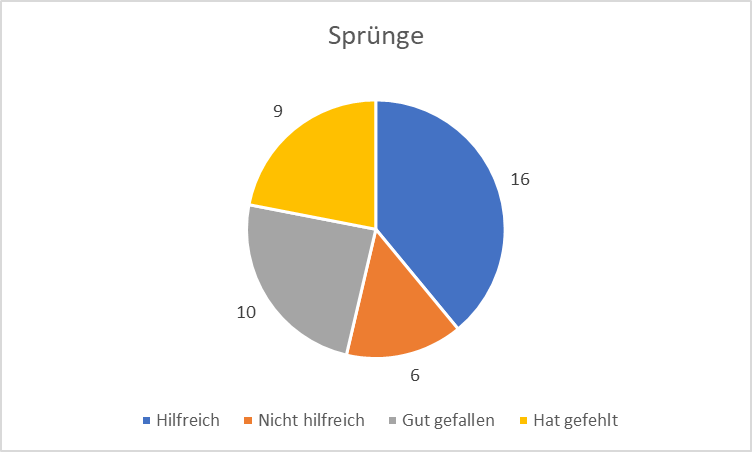
\includegraphics[width=\linewidth]{pictures/diagramme/aussagenspr}
      \caption{caption}
   \end{minipage}
   \hspace{.01\linewidth}% Abstand zwischen Bilder
   \begin{minipage}[b]{.49\linewidth} % [b] => Ausrichtung an \caption
      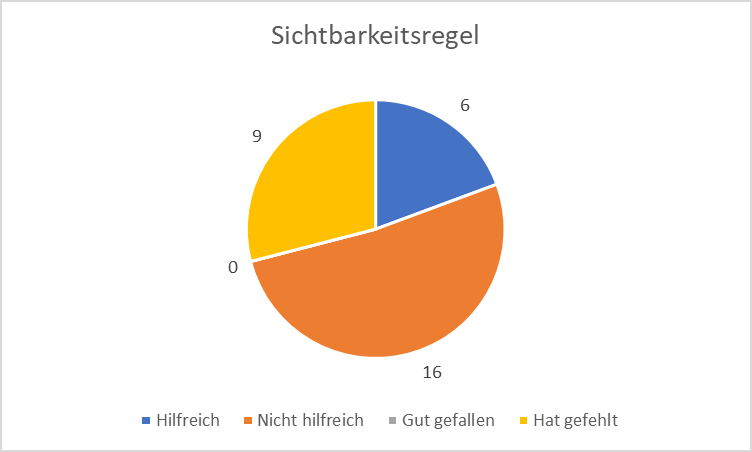
\includegraphics[width=\linewidth]{pictures/diagramme/aussagensichtb}
      \caption{caption}
   \end{minipage}
\end{figure}

\paragraph{Verständlichkeit der Konversationsdarstellung}
Hinsichtlich der Darstellung der Konversationen lässt sich eine Tendenz feststellen, die aufzeigt, dass diese im \emph{TherapyBuilder}-Prototyp verständlicher dargestellt sind. Betrachtet man die Ergebnisse der Studie der einzelnen Prototypen, so lässt sich die Tendenz folgendermaßen begründen. Da die Konversation einem ähnlichen Format folgt, wie es in herkömmlichen Chat-Technologien eingesetzt wird, ist die Konversation besser nachzuvollziehen. Diese Aussagen finden sich in der Abschlussfragerunde wieder. Die Freitext-Aussagen merken an, dass die zeitliche Abfolge, wie auch die Gestaltung, zum besseren Verständnis des Konversationsablaufs beitragen. Im Vergleich zur entsprechenden Umsetzung der Konversationsdarstellung, mit Hilfe von Sprüngen, vermissen die Probanden allgemein die Übersichtlichkeit des Konversationsverlaufs. Ein Proband merkt diesbezüglich an, dass es anhand des in \emph{movisensXS} verwendeten Formats, schwer nachvollziehbar ist, wie die Konversation letztendlich auf dem Smartphone des Nutzers aussehen wird. Diese Aussagen ließen sich ebenfalls in der Abschlussfragerunde finden. 

Das Format der Konversationsdarstellung wurde im \emph{TherapyBuilder} für den Nutzer verständlicher umgesetzt. Das eingesetzte Format des \emph{movisensXS}-Prototyps, könnte dahingehend durch eine räumliche und farbliche Trennung der Chatbot-Ausgaben verbessert werden. Auch die Sichtbarkeitsregeln klarer darzustellen und den damit einhergehenden Verlauf abzubilden, könnte die Verständlichkeit der Darstellung verbessern.

\paragraph{Verständlichkeit der Konversationseinstellungen}
Die Einstellungsmöglichkeiten der Konversationen wurde von den Probanden folgendermaßen bewertet. Im Vergleich schneidet der \emph{movisensXS}-Prototyp in diesem Punkt schlechter ab, als der \emph{TherapyBuilder}-Prototyp. Hinsichtlich der Einstellungsmöglichkeiten innerhalb der Darstellung mit Sprüngen hoben die Probanden folgende Punkte positiv hervor. Zwar gibt es viele Einstellungsmöglichkeiten, diese erschlagen visuell allerdings nicht. Außerdem ist auf einen Blick ersichtlich, wann und wie eine Verzweigung stattfindet und zu welchem Zeitpunkt man sich um den Sprung innerhalb des Konversationsverlaufs kümmern muss. Allerdings musste das Bauelement für die Einstellung des Sprungs, lange gesucht werden. Außerdem benötigt es zunächst ein Gefühl für die Einstellung des Sprungs. Auch die Erweiterbarkeit der Lanes ist klar. Eine Anleitung, farbliche Unterscheidung des Sprung-Elements, sowie Tooltips, könnten dabei Helfen den Sprung einzubauen und zu konfigurieren. Betrachtet man die Daten hinsichtlich der Sichtbarkeitsregeln, die der \emph{movisensXS}-Prototyp verwendet, zeichnet sich hier dennoch eine Tendenz ab, dass die Einstellung der Sprünge verständlicher ist. Die Anzahl der Elemente, die verwendet werden können um eine Konversation zusammen zu bauen, ist in beiden Prototypen die gleiche, bis auf das zusätzliche Element, welches die Sprünge steuert. Interessant ist, dass ein paar Probanden die Vielfalt dieser Elemente im \emph{movisensXS} positiv hervorgehoben haben. Dies lässt vermuten, dass ihnen hier die Anzahl der Elemente größer erscheint. Auch hier wurde die Drag and Drop-Funktion positiv angemerkt. Allerdings vermissen auch hier die Probanden eine Bedienungsanleitung beispielsweise um den Nutzer besser heranzuführen. Das Auge irritiert bei den Einstellungen eher, auch wenn zwei Probanden damit gut zurecht kamen, da ihnen dieses Prinzip in Form eines Filters bereits von einem Programm namens \emph{Redcap} bekannt ist. Die Probanden äußerten mehrheitlich, dass das Auge irritiert und unter geht, da es sich erst offenbart, sobald man die Maus über ein Element innerhalb des Konversationsverlaufs bewegt. Wurde einem Element eine Regel hinterlegt, wird dies nur durch das Anzeigen des Auges verdeutlicht. Zwar sieht man auf diese Weise, dass etwas hinterlegt ist, allerdings, so sagen die Probanden, erkennt man nicht die Auswirkungen dessen. Diesen muss man sich im Gedächtnis behalten oder immer wieder neu einsehen. Der kognitive Aufwand ist somit sehr hoch. Auch bei der Einstellung der Sichtbarkeitsregel macht sich dies bemerkbar. So sind Variablen, anhand derer man die Sichtbarkeit eines Elements steuern möchte, nicht auf einen Blick einsehbar. Der Nutzer muss sich vergewissern, dass die entsprechende Variable existiert und den exakten Variablennamen merken. Hier herrscht eine hohe Fehleranfälligkeit. Ist eine Regel nicht valide, so wird das gesamte Element rot eingefärbt. Dies erschwert allerdings das Löschen der Regel. Das Icon für diese Funktion ist ebenfalls rot und sticht in diesem Fall farblich nicht mehr hervor und ist somit schwer zu finden.

Die Einstellungsmöglichkeiten des \emph{TherapyBuilder}-Prototyps, zur Erstellung von Konversationen mit Sprüngen, ist demnach tendenziell verständlicher. Diese könnte man allerdings durch den Einsatz von Anleitungen, Tooltips und einer farblich stärkeren Trennung der Elemente, beispielsweise um das Sprung-Element sichtbarer zu gestalten, verbessern. Die Einstellungsmöglichkeiten des \emph{movisensXS} könnten durch eine Visualisierung der Auswirkungen, der zeitlichen Abbildung sowie einer besseren Trennung der Elemente durch räumliche und farbliche Trennung verständlicher gestaltet werden. Außerdem könnte eine Übersicht der vorhandenen Variablen helfen, die kognitive Belastung zu verringern. Icons sollten sich auch bei Fehlermeldungen innerhalb eines Elements hervorheben um diese für den Nutzer sichtbarer zu gestalten. Das generelle Einstellung einer Regel könnte durch eine andere Form der Darstellung verbessert werden. Die Funktion könnte beispielsweise dauerhaft angezeigt werden. Ist eine Regel hinterlegt, könnten Linien beispielsweise darstellen, auf welche Elemente sich diese Regel auswirkt.


\paragraph{Übersichtlichkeit des Konversationsverlaufs}
Die Bewertungen und Aussagen der Probanden zeigen auf, dass die Darstellung des Konversationsverlaufs innerhalb des \emph{movisensXS}-Prototyps tendenziell unübersichtlicher gestaltet ist. Die Probanden gaben diesbezüglich an, dass der zeitliche Verlauf schwer nachvollziehbar sei. Der \emph{TherapyBuilder}-Prototyp hingegen hat eine klare Struktur des Gesprächsverlaufs wodurch dieser gut nachvollziehbar ist. Insbesondere die Sprünge und die verwendeten Lanes tragen dazu bei. Diese sind durch die gewählte Darstellung offensichtlicher und besser sichtbar. Auch die Darstellung der Elemente in einem Format, welches an bekannte Chat-technologien angelehnt ist, trägt dazu bei. Allerdings wurde angemerkt, dass die Nachvollziehbarkeit der Sprünge durch eine leicht veränderte Anordnung verbessert werden könnte.

Die Darstellungsform des \emph{movisensXS}-Prototyps könnte in diesem Punkt verbessert werden. Während die Sprünge durch eine farbliche Kodierung und einer mittigen Platzierung des Hauptstrangs der Konversation verbessert werden könnte, wäre eine Visualisierung der Sichtbarkeitsregeln und ihrer Auswirkungen hilfreich. Auch eine farbliche Unterscheidung der Chatbot-Output und Patient-Input Elemente könnten eine bessere Übersicht über den Konversationsverlauf bieten. Möglich wäre auch eine kleine Live-Vorschau darüber, wie der Patient die Konversation innerhalb der Smartphone-App zu sehen bekommt. Dies könnte die Übersichtlichkeit des Konversationsverlaufs und der Sichtbarkeitsregeln verbessern. 

\paragraph{Übersichtlichkeit der Antwortoptionen innerhalb des Konversationsverlaufs}
Betrachtet man zunächst die Fragebogenauswertung in Abbildung \ref{antwortendurchsch22}, lässt diese vermuten, dass die Antwortoptionen innerhalb des Konversationsverlaufs besonders Übersichtlich im \emph{TherapyBuilder}-Prototyp abgebildet wurde. Allerdings lässt sich dies nicht anhand der Freitext-Angaben und gegebenen Antworten der Abschlussfragerunde genau begründen.

Aufgrund der fehlenden Aussagen, die sich auf die Übersichtlichkeit der Antwortoptionen innerhalb des Konversationsverlaufs beziehen, kann hier keine genaue Tendenz festgelegt und keine Begründung gegeben werden. 

\paragraph{Verständlichkeit der Verzweigungen innerhalb des Konversationsverlaufs}
Die Sichtbarkeitsregeln wurden im Fragebogen hinsichtlich der Verständlichkeit innerhalb des Konversationsverlaufs schlechter bewertet als die Sprünge. Nicht nur die Freitexte des Fragebogens geben einen Hinweis darauf. Die Begründung der schlechteren Bewertung lassen sich darin finden, dass die Sichtbarkeitsregeln, die den Dialogfluss steuern, schwer zu finden sind. Die Andeutung durch das Icon ist zunächst verwirrend. Ist die Funktion klar, kann nur eingesehen werden, an welcher Stelle eine Regel hinterlegt wurde. Die genaue Abfolge ist nicht ersichtlich. Wurden mehrere Sichtbarkeitsregeln an mehreren Elementen hinterlegt, so ist der Verlauf schnell unklar. Die Darstellung der Sprünge mit Pfaden und Lanes ist generell gut verständlich. Wie verständlich diese letztendlich bei höherer Komplexität und vielfachen Sprüngen mit mehreren Lanes muss zunächst noch genauer betrachtet werden. 

Die Sichtbarkeitsregel könnte verbessert werden indem das entsprechende Icon beispielsweise immer sichtbar bleibt. Wurde eine Regel hinterlegt, könnte durch den Einsatz von Pfaden, der Bezug zu verschiedenen Elementen dargestellt werden. Auch eine kleine Übersicht des Konversationsverlaufs aus Patienten-Sicht könnte helfen die Verzweigungen sichtbarer und verständlicher zu machen.

\paragraph{Übersichtlichkeit der Werkzeugpalette zur Konversationserstellung}
Anhand der Ergebnisse des Fragebogens und der Abschlussfragerunde, zeigt sich hier, dass die Probanden den \emph{TherapyBuilder}-Prototyp in diesem Punkt besser bewerteten. Die Freitexte des Fragebogens und Ergebnisse der Abschlussfragerunde geben nicht die in Abbildung \ref{antwortendurchsch22} angedeutete Tendenz wieder. Der \emph{TherpayBuilder}-Prototyp gibt, beim  Öffnen des Konversationsverlaufs, eine bessere Übersicht der Werkzeugpalette. Zu diesem Zeitpunkt werden die drei Kategorien \emph{Patient Input}, \emph{Chatbot-Output} und \emph{Control Logic} aufgelistet. Erst wenn der Nutzer auf diese klickt, öffnet sich die entsprechende Kategorie, die entsprechende Elemente preisgibt. Der \emph{movisensXS}-Prototyp verwendet zwar eine ähnliche Kategorisierung, allerdings werden beim Aufrufen der Konversation bereits alle Elemente angezeigt. Die Kategorisierung wird hier leicht übersehen. Allerdings wurde das Element, welches die Sprünge darstellt und konfiguriert, innerhalb der Werkzeugpalette des \emph{TherapyBuilder}-Prototyps lange gesucht. 

Die Bedienung und das Zusammensetzen der Konversation fiel den Probanden insgesamt in beiden Ansätzen leicht. Dennoch könnten Tooltips und eine Anleitung beide Ansätze verbessern. Insbesondere hinsichtlich der Einstellung der Sichtbarkeitsregeln und Sprünge. 


\subsection{Zusammenfassung}
Insgesamt wurde der \emph{TherapyBuilder}-Prototyp in der Studie besser bewertet. Auch zeigt sich eine Tendenz, dass die Konzepte die aufgestellten Hypothesen, aus Kapitel \ref{ch:evaluation}, belegt werden könnten. Das Konfigurationsprinzip ist insgesamt besser verständlich und übersichtlicher. Allerdings schneidet es in der Einstellung der Trigger schlechter ab. Hier sticht das \emph{Konstruktionsprinzip} besonders durch das Baukastenprinzip hervor. Die dort angebotenen Bausteine sind nach ihrer Funktion kategorisiert und farblich kodiert. Die farbliche Kodierung unterstützt die sinnvolle Anordnung der Bausteine und bringt außerdem eine Ordnung in die entstehende Baumstruktur. Die damit einhergehende Flexibilität der Gestaltung hebt sich besonders positiv hervor. Allerdings ist die Anordnung von mehreren Elementen schnell unübersichtlich. Der zeitliche Verlauf ist schwer nachvollziehbar. Die getriggerten Konversationen sind schwer zu überblicken. Diese müssen händisch gesucht werden. Das Konfigurationsprinzip hingegen ist schwer nachvollziehbar bezüglich der Konfiguration der Triggereinstellungen. Außerdem benötigt die zeitliche Darstellung eine aussagekräftigere Legende und Tooltips, die einfache Erklärungen der vorhandenen Funktionen bieten. Das Konfigurationsprinzip könnte von den positiven Eigenschaften des Konstruktionsprinzips profitieren. Die Trigger-Einstellungen einer Konversation könnten sich beispielsweise durch eine Anlehnung an das Konstruktionsprinzip realisieren lassen. Statt einen Baum zu erstellen, der den gesamten Therapieablauf abbildet, könnte in den Trigger-Einstellungen einer Konversation ein kleiner Baum erstellt werden. Dieser ist entsprechend nur für diese Konversation repräsentativ. Ähnlich strikte Regeln für die Anordnung könnten hierbei helfen, diesen Baum innerhalb der Timeline abzubilden. So wäre die zeitliche Übersicht des Therapieverlaufs noch immer gegeben. Das Konstruktionsprinzip könnte von einer strengeren Anordnung profitieren. Beispielsweise durch den Einsatz von Spalten um eine zeitliche Übersicht abzubilden und die Suche nach Konversationen zu erleichtern. Auch könnte eine Suchfunktion für einzelne Konversationen hilfreich sein um längeres Suchen im Baum zu vermeiden.

Die Übersichtlichkeit und Verständlichkeit der Sprünge ist ebenfalls tendenziell besser im Vergleich zu den Sichtbarkeitsregeln. Bei letzteren ist der einhergehende Verlauf der Konversation schwer nachzuvollziehen. Die Augen-Metapher ist nicht ganz eindeutig und versteckt. Die Patienten-Eingabe hebt sich visuell kaum von der Chatbot-Ausgabe ab. Die Werkzeugpalette könnte von einer visuell besseren Trennung der Chatbot-Output und Patient-Input Elemente profitieren. Auch die Einstellung der Sichtbarkeitsregeln könnte verbessert werden. Zum einen könnte die Funktion dauerhaft sichtbar dargestellt werden. Eine kleine Vorschau des Konversationsablaufs aus Nutzersicht könnte einen besseren Überblick der Konversation und den Abhängigkeiten geben. Die Sprünge hingegen sind visuell gut nachvollziehbar. Das Einbauen der Sprünge könnte durch eine farbliche Unterscheidung vereinfacht werden. Die Verwendung und Einstellung der Sprünge, als auch der Sichtbarkeitsregeln, können durch eine Anleitung und Tooltips verbessert werden.


\section{Kritische Reflexion}
Insgesamt zeigen sich nach der Durchführung der Studie einige Tendenzen hinsichtlich des Vergleichs der betrachteten Konzepte. Allerdings können die Hypothesen auf der erhobenen Datenbasis nicht bestätigt werden. Hierfür benötigt es mehr Probanden um die Konzepte ausreichend zu vergleichen. Auch zeigt sich, dass die Studie in wenigen Punkten Anpassungen benötigt. So konnte die Übersichtlichkeit der Antwortoptionen innerhalb des Konversationsverlaufs nicht vollständig betrachtet werden, da die Probanden diese zwar in den Fragebögen bewerteten, allerdings trafen sie hinsichtlich dieser Hypothese keine Aussagen. Auf diese könnte der Studienleiter während der Aufgabenbearbeitung und innerhalb der Abschlussfragerunde intensiver eingehen und den Probanden stärker anleiten. Dennoch konnten viele Daten erhoben werden, die Stärken und Schwächen beider Systeme aufzeigen und zu einer Verbesserung der Konzepte beitragen können. Auch können die erhobenen Daten zu einer Verbesserung des handelsüblichen \emph{movisensXS} System beitragen um die Verständlichkeit und Übersichtlichkeit zu verbessern. 

Während der Durchführung der Studie wurden außerdem Videoaufnahmen des Desktops sowie des Probanden, in Bild und Ton, angefertigt. Diese Daten könnten zusätzlich ausgewertet und in die Interpretation mit eingebracht werden. So könnten beispielsweise die Bearbeitungszeiten einzelner Aufgaben interessant sein. Aber auch weitere Äußerungen während der Aufgabenbearbeitung und Blickfolgen, könnten interessante Daten liefern und weitere Probleme oder positiven Aspekte aufdecken.

